\documentclass[10pt,a4paper]{article}
\usepackage[UTF8,fontset = windows]{ctex}
\setCJKmainfont[BoldFont=黑体,ItalicFont=楷体]{华文中宋}
\usepackage{amssymb,amsmath,amsfonts,amsthm,mathrsfs,dsfont,graphicx}
\usepackage{ifthen,indentfirst,enumerate,color,titletoc}
\usepackage{tikz}
\usepackage{multicol}
\usepackage{makecell}
\usepackage{longtable}
\usetikzlibrary{arrows,calc,intersections,patterns,decorations.pathreplacing,3d,angles,quotes,positioning}
\usepackage[bf,small,indentafter,pagestyles]{titlesec}
\usepackage[top=1in, bottom=1in,left=0.8in,right=0.8in]{geometry}
\renewcommand{\baselinestretch}{1.65}
\newtheorem{defi}{定义~}
\newtheorem{eg}{例~}
\newtheorem{ex}{~}
\newtheorem{rem}{注~}
\newtheorem{thm}{定理~}
\newtheorem{coro}{推论~}
\newtheorem{axiom}{公理~}
\newtheorem{prop}{性质~}
\newcommand{\blank}[1]{\underline{\hbox to #1pt{}}}
\newcommand{\bracket}[1]{(\hbox to #1pt{})}
\newcommand{\onech}[4]{\par\begin{tabular}{p{.9\textwidth}}
A.~#1\\
B.~#2\\
C.~#3\\
D.~#4
\end{tabular}}
\newcommand{\twoch}[4]{\par\begin{tabular}{p{.46\textwidth}p{.46\textwidth}}
A.~#1& B.~#2\\
C.~#3& D.~#4
\end{tabular}}
\newcommand{\vartwoch}[4]{\par\begin{tabular}{p{.46\textwidth}p{.46\textwidth}}
(1)~#1& (2)~#2\\
(3)~#3& (4)~#4
\end{tabular}}
\newcommand{\fourch}[4]{\par\begin{tabular}{p{.23\textwidth}p{.23\textwidth}p{.23\textwidth}p{.23\textwidth}}
A.~#1 &B.~#2& C.~#3& D.~#4
\end{tabular}}
\newcommand{\varfourch}[4]{\par\begin{tabular}{p{.23\textwidth}p{.23\textwidth}p{.23\textwidth}p{.23\textwidth}}
(1)~#1 &(2)~#2& (3)~#3& (4)~#4
\end{tabular}}
\begin{document}

\begin{enumerate}[1.]

\item {\tiny (003501)}用``$\subseteq$''连接集合$\mathbf{Z}$、$\mathbf{Q}$、$\mathbf{R}$、$\mathbf{C}$:\blank{50}.
\item {\tiny (002697)}设全集$U=\{2,3,a^2+2a-3\}$, 集合$A=\{|2a-1|,2\}$, $\overline A=\{5\}$, 则实数$a=$\blank{50}.
\item {\tiny (002712)}设集合$A\cap \{-2,0,1\}=\{0,1\}$, $A\cup \{-2,0,2\}=\{-2,0,1,2\}$, 则满足上述条件的集合$A$的个数为\blank{50}个.
\item {\tiny (002703)}设全集$U=\mathbf{R}$, 函数$y=f(x)$, $y=g(x)$, $y=h(x)$的定义域均为$\mathbf{R}$. 设集合$A=\{x|f(x)=0\}$, $B=\{x|g(x)=0\}$, $C=\{x|h(x)=0, \ x\in \mathbf{R}\}$, 则方程$\dfrac{f^2(x)+g^2(x)}{h(x)}=0$的解集是\blank{50}(用$A,B,C$表示).
\item {\tiny (001014)}已知集合$M=\{y|y=x+1, \ x \in \mathbf{R}\}$, $N=\{y|y=-x^2+4x,\  x \in \mathbf{R}\}$,
则$M \cap N=$\blank{80}.
\item {\tiny (004794)}已知非空集合$P$满足: \textcircled{1} $P\subseteq \{1,2,3,4,5\}$; \textcircled{2} 若$a\in P$, 则$6-a\in P$. 符合上述要求的集合P的个数是\bracket{20}.
\fourch{$4$}{$5$}{$7$}{$31$}
\item {\tiny (020065)}用集合$A$、$B$的运算式表示图中的阴影部分:\\
(1) 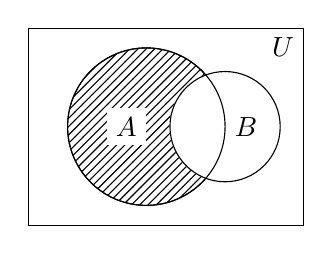
\begin{tikzpicture}
\draw (0,0) rectangle (3.5,2.5) node [below left] {$U$};
\filldraw [pattern = {north east lines}] (1.5,1.25) circle (1);
\filldraw [white] (2.5,1.25) circle (0.7);
\draw (1.5,1.25) circle (1) node [left, fill = white] {$A$};
\draw (2.5,1.25) circle (0.7) node [right] {$B$};
\end{tikzpicture}
(2) 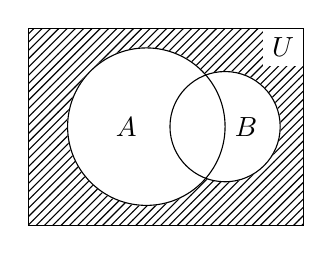
\begin{tikzpicture}
\filldraw [pattern = {north east lines}] (0,0) rectangle (3.5,2.5);
\draw (0,0) rectangle (3.5,2.5) node [below left, fill = white] {$U$};
\filldraw [white] (1.5,1.25) circle (1);
\filldraw [white] (2.5,1.25) circle (0.7);
\draw (1.5,1.25) circle (1) node [left] {$A$};
\draw (2.5,1.25) circle (0.7) node [right] {$B$};
\end{tikzpicture}
(3) 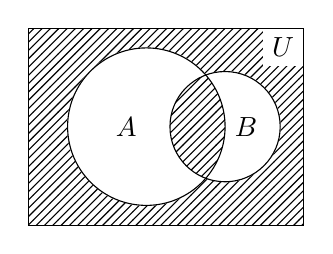
\begin{tikzpicture}
\filldraw [pattern = {north east lines}] (0,0) rectangle (3.5,2.5);
\draw (0,0) rectangle (3.5,2.5) node [below left, fill = white] {$U$};
\filldraw [white] (1.5,1.25) circle (1);
\filldraw [white] (2.5,1.25) circle (0.7);
\begin{scope}
    \clip (1.5,1.25) circle (1);
    \clip (2.5,1.25) circle (0.7);
    \filldraw [pattern = {north east lines}] (0,0) rectangle (3.5,2.5);
\end{scope}
\draw (1.5,1.25) circle (1) node [left] {$A$};
\draw (2.5,1.25) circle (0.7) node [right] {$B$};
\end{tikzpicture}
\vspace*{4ex}
\item {\tiny (020028)}已知集合$A=\{1\}$, $B=\{x|x\subseteq A\}$, 用列举法表示集合$B$. 并指出$A$与$B$的关系.
\vspace*{4ex}
\item {\tiny (001016)}已知集合$A=\{1,2\}$, $B=\{x|mx^2+2mx-1<0, x \in\mathbf{R}\}$. 已知$A \cap B=\{1\}$, 求实数$m$的取值范围.
\vspace*{8ex}
\item {\tiny (010026)}已知集合$A=\{2, (a+1)^2, a^2+3a+3\}$, 且$1\in A$. 求实数$a$的值.
\vspace*{8ex}
\item {\tiny (020034)}已知集合$S=\{1, 2\}$, 集合$T=\{x|ax^2-3x+2=0\}$, 且$S\supseteq T$, 求实数$a$的取值范围.
\vspace*{8ex}
\item {\tiny (004770)}已知$a$是实常数, 集合$A=\{x|x^2-5x+4\le 0\}$与$B=\{x|x^2-2ax+a+2\le 0\}$满足$B\subseteq A$, 求$a$的取值范围.
\vspace*{16ex}
\item {\tiny (020040)}已知集合$A=\{1, 1+d, 1+3d\}$, 集合$B=\{1, q, q^2\}$, 其中$d$、$q\in \mathbf{R}$, 且$d\ne 0$. 若$A=B$, 求$q$的值.
\vspace*{20ex}
\item {\tiny (010021)}已知集合$A=\{1\}$, $B=\{x|x^2-3x+a=0\}$. 是否存在实数$a$, 使得$A\subset B$?  若存在, 求$a$的值; 若不存在, 说明理由.
\vspace*{20ex}
\item {\tiny (002700)}集合$C=\{x|x=\dfrac k2\pm \dfrac14, \ k\in \mathbf{Z}\},D=\{x|x=\dfrac k4,\ k\in \mathbf{Z}\}$, 试判断$C$与$D$的关系, 并证明.
\vspace*{24ex}
\item {\tiny (020041)}已知$A=\{x|x=a+\sqrt 2b,\ a,b\in \mathbf{N}\}$, 若集合$B=\{x|x=\sqrt 2x_1,\  x_1 \in A\}$, 证明$B\subset A$.
\vspace*{24ex}
\end{enumerate}



\end{document}